\newpage
%
% Návrh
%
\ifthenelse {\boolean{bachelor}}
{
	%\section{Design}
	\section{Návrh}
}
{
	%\chapter{Design}
	\chapter{Návrh}
}
\label{section:design}

%
% Návrh uchovávania textov v databázach
%
\ifthenelse {\boolean{bachelor}}
{
	%\subsection{Subsection}
	\subsection{Návrh uchovávania textov v databázach}
}
{
	%\section{Subsection}
	\section{Návrh uchovávania textov v databázach}
}
\label{subsection:our_design_persisting_data}
Na uchovávanie dát sme zvolili dokumentovú databázu MongoDB. Ukladané dáta sa dajú rozdeliť do niekoľkých samostatných kolekcií. Sú to:

\begin{my_itemize}
	\myitem rules,
	\myitem sentences,
	\myitem notes
	\myitem structures,
	\myitem articles,
	\myitem and rules.
\end{my_itemize}
	
Prepojenia medzi jednotlivými kolekciami sú zobrazené na obrázku~\fullref{fig:db_schema}. Nasledujúcich časti opisujú stručne každú kolekciu. Všetky kolekcie obsahujú okrem polí špecifických pre danú kolekciu, aj polia časových značiek označujúcich vytvorenie a aktualizáciu záznamu.

\begin{figure}[H]
	\begin{center}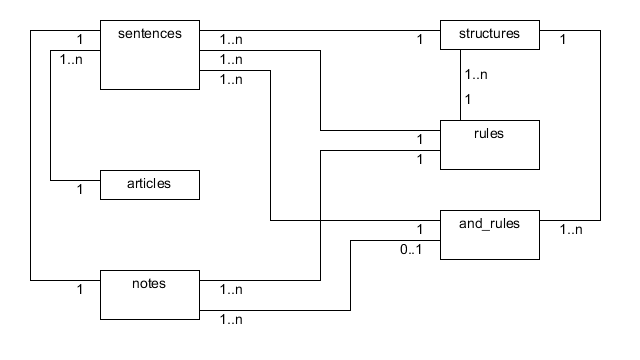
\includegraphics[scale=0.60]{db_schema}\end{center}
	\caption[Databázový model]{Databázový model}\label{fig:db_schema}
\end{figure}

%
% Kolekcia texts
%
\ifthenelse {\boolean{bachelor}}
{
	%\subsection{Subsection}
	\subsubsection{Kolekcia articles}
}
{
	%\section{Subsection}
	\subsection{Kolekcia articles}
}
\label{subsubsection:collection_articles}
V kolekcií \textit{articles} sa ukladajú spracovávané texty. 

Kolekcia obsahuje textové pole \textit{text} na uloženie textu v pôvodnom tvare. Model kolekcie \textit{articles} je zobrazený na obrázku~\fullref{fig:articles_collection_model}.

\begin{figure}[H]
	\begin{center}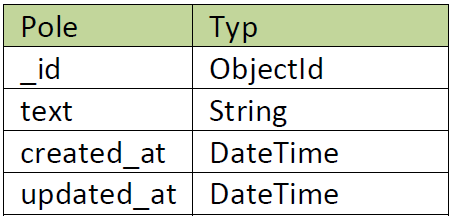
\includegraphics[scale=0.60]{articles_model}\end{center}
	\caption[Model kolekcie articles]{Model kolekcie articles}\label{fig:articles_collection_model}
\end{figure}

%
% Kolekcia notes
%
\ifthenelse {\boolean{bachelor}}
{
	%\subsection{Subsection}
	\subsubsection{Kolekcia notes}
}
{
	%\section{Subsection}
	\subsection{Kolekcia notes}
}
\label{subsubsection:collection_notes}
Kolekcia \textit{notes} uchováva vytvorené poznámky z viet.

Obsahuje textové pole \textit{text} s hodnotou poznámky a dve referencujúce polia. Jedno sa odkazuje do kolekcie \textit{rules} na pravidlo, ktoré bolo použité na vytvorenie poznámky. Druhé referencuje použité and\hyph pravidlo v kolekcií \textit{and\textunderscore rules}. Toto pole môže byť prázdne, ak sa and\hyph pravidlo pri vytváraní poznámky nepoužilo. Na obrázku~\fullref{fig:notes_collection_model} je vyobrazený model kolekcie \textit{notes}.

\begin{figure}[H]
	\begin{center}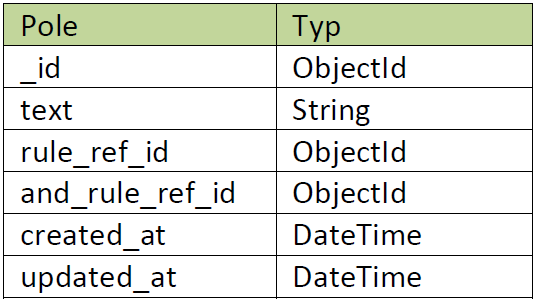
\includegraphics[scale=0.60]{notes_model}\end{center}
	\caption[Model kolekcie notes]{Model kolekcie notes}\label{fig:notes_collection_model}
\end{figure}

%
% Kolekcia sentences
%
\ifthenelse {\boolean{bachelor}}
{
	%\subsection{Subsection}
	\subsubsection{Kolekcia sentences}
}
{
	%\section{Subsection}
	\subsection{Kolekcia sentences}
}
\label{subsubsection:collection_sentences}
V následujúcej kolekcií \textit{sentences} sa ukladajú spracované vety aj s informáciami o článku, pravidlách a poznámke.

Kolekcia sa skladá z textového polia \textit{text} uchovávajúce hodnotu vety a piatich referencujúcich polí \textit{article\textunderscore ref\textunderscore id}, \textit{structure\textunderscore ref\textunderscore id}, \textit{rule\textunderscore id}, \textit{rule\textunderscore ref\textunderscore id}, \textit{and \textunderscore rule\textunderscore ref\textunderscore id} a \textit{note\textunderscore id}. \textit{Article\textunderscore ref\textunderscore id} odkazuje na článok z kolekcie \textit{articles}, ktorého súčasťou je daná veta. Pole \textit{structure\textunderscore ref\textunderscore id} odkazuje do kolekcie \textit{structures}, ktoré reprezentuje štruktúru vety. Nasledujúce polia \textit{rule\textunderscore ref\textunderscore id} a \textit{and\textunderscore rule\textunderscore ref\textunderscore id} odkazujú na použité pravidlo a and\hyph pravidlo pri spracovávaní vety, v tomto poradí. Pole \textit{note\textunderscore ref\textunderscore id} odkazuje na poznámku z kolekcie \textit{notes}, ktorá bola vytvorená z vety.

Model tejto kolekcie je načrtnutý na obrázku~\fullref{fig:sentences_collection_model}.

\begin{figure}[H]
	\begin{center}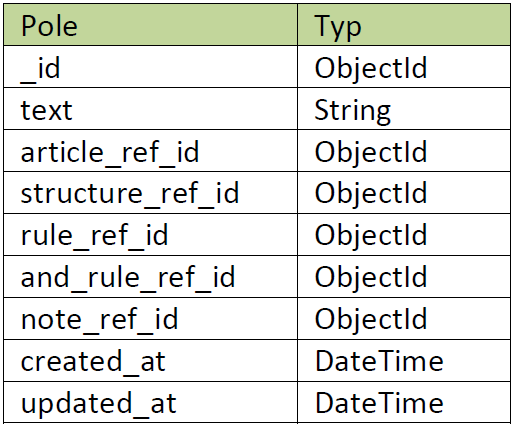
\includegraphics[scale=0.60]{sentences_model}\end{center}
	\caption[Model kolekcie sentences]{Model kolekcie sentences}\label{fig:sentences_collection_model}
\end{figure}

%
% Kolekcia structures
%
\ifthenelse {\boolean{bachelor}}
{
	%\subsection{Subsection}
	\subsubsection{Kolekcia structures}
}
{
	%\section{Subsection}
	\subsection{Kolekcia structures}
}
\label{subsubsection:collection_structures}
V kolekcií \textit{structures} sú uložené štruktúry viet a pravidiel. Štruktúra je zložená hlavne zo závislostí, tokenov, názvoslovných značiek, indexov a iné.

Kolekcia sa skladá z jedného pola \textit{structure\textunderscore data}. Toto pole je zoznam dokumentov, obsahujúcich vyššie spomenuté údaje. Dokument v tomto zozname obsahuje textové pole \textit{relation\textunderscore name} s názvom vzťahu závislosti a zoznam dokumentov závislostí \textit{dependencies} s týmto názvom vzťahu. Dokument v zozname \textit{dependencies} sa skladá z polí \textit{governor} a \textit{dependent} typu dokument, celočíselného pola \textit{position} uchovávajúceho pozíciu závislosti vo vete alebo poznámke, \textit{comparison\textunderscore type}, ktoré je celočíselnou reprezentáciou typu porovnania a poľa \textit{token\textunderscore type}, ktoré je taktiež celočíselnou reprezentáciou typu tokenu. Dokumenty polí \textit{governor} a \textit{depdendent} obsahujú údaje o prislúchajúcich tokenoch závislosti. V textovom poli \textit{POS} sa ukladá značka slovného druhu, pole \textit{index} uchováva index tokenu vo vete, \textit{ner} je textové pole reprezentujúce názvoslovnú entitu tokenu a v poli \textit{lemma} je textová reprezentácia lemy tokenu.

Celý model kolekcie je zobrazený na obrázku~\fullref{fig:structures_collection_model}.

\begin{figure}[H]
	\begin{center}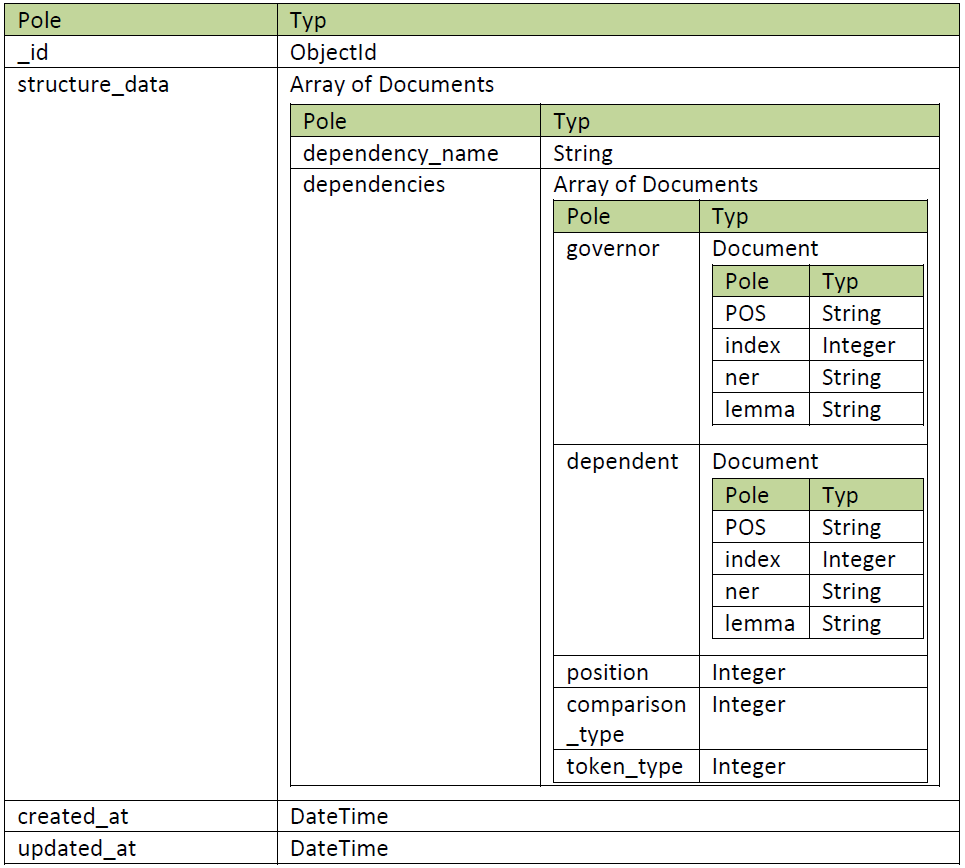
\includegraphics[scale=0.53]{structure_model}\end{center}
	\caption[Model kolekcie structures]{Model kolekcie structures}\label{fig:structures_collection_model}
\end{figure}

%
% Kolekcia rules
%
\ifthenelse {\boolean{bachelor}}
{
	%\subsection{Subsection}
	\subsubsection{Kolekcia rules}
}
{
	%\section{Subsection}
	\subsection{Kolekcia rules}
}
\label{subsubsection:collection_rules}
\textit{Rules} je kolekcia, do ktorej sa ukladajú pravidla na vytvorenie poznámok z viet. Vďaka databázovému modelu na obrázku~\fullref{fig:db_schema} a prepojeniam medzi kolekciami je táto kolekcia minimalistická.

Skladá sa z dvoch polí. Pole \textit{sentence\textunderscore terminators} je zoznam čísel, ktoré reprezentujú konce viet v poznámke. Referencujúce pole \textit{structure\textunderscore ref\textunderscore id} odkazuje do kolekcie \textit{structures} na štruktúru, ktorou sa má prípadná veta spracovať. Model kolekcie \textit{rules} je vyjadrený obrázkom~\fullref{fig:rules_collection_model}.

Pole \textit{sentence\textunderscore terminators} zväčša obsahuje jeden záznam. Napríklad pri vete \textit{,,The president of the Slovak Republic is andrej Kiska.''} a poznámke z tejto vety v tvare \textit{,,President is Kiska.''} bude obsahovať jeden záznam: 3. Číslo 3 preto, lebo koniec vety, v tomto prípade bodka, sa nachádza na tretej pozícií spomedzi tokenov vo vete. Číslovanie pozícií začína  m nula. V prípade ak veta je súvetie, zložené z viacerých jednoduchých viet, môže pole \textit{sentence\textunderscore terminators} obsahovať viacero záznamov, ak napríklad chceme z každej jednoduchej vety súvetia získať zjednodušenú vetu a vytvoriť tak zloženú poznámku, skladajúcu sa zo zjednodušených viet.

\begin{figure}[H]
	\begin{center}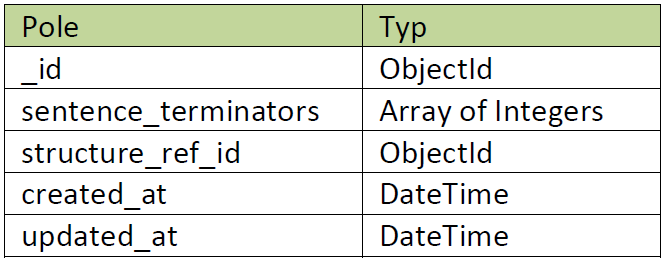
\includegraphics[scale=0.60]{rules_model}\end{center}
	\caption[Model kolekcie rules]{Model kolekcie rules}\label{fig:rules_collection_model}
\end{figure}

%
% Kolekcia and_rules
%
\ifthenelse {\boolean{bachelor}}
{
	%\subsection{Subsection}
	\subsubsection{Kolekcia and rules}
}
{
	%\section{Subsection}
	\subsection{Kolekcia and rules}
}
\label{subsubsection:collection_and_rules}
Posledná kolekcia uchováva pravidlá pre spracovanie vety a vytvorenie viacnásobnej poznámky z vety. Táto kolekcia je veľmi podobná kolekcií \textit{rules} a obsahuje rovnaké polia doplnené o ďalšie špecifické pole.

Špecifické pole, o ktoré je kolekcia rozšírená oproti kolekcií \textit{rules} je celočíselné pole \textit{set\textunderscore position}. Toto pole uchováva pozíciu množiny v viacnásobnej poznámke. Model kolekcie je vyobrazený na obrázku~\fullref{fig:and_rules_collection_model}.

\begin{figure}[H]
	\begin{center}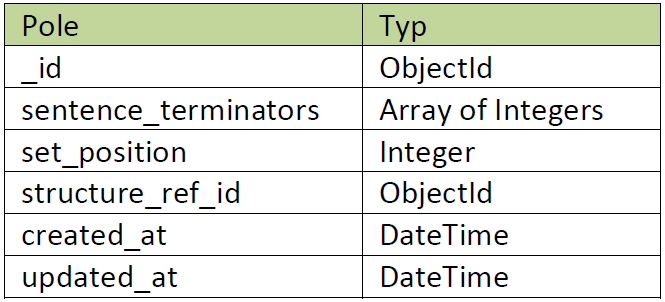
\includegraphics[scale=0.60]{and_rules_model}\end{center}
	\caption[Model kolekcie and rules]{Model kolekcie and rules}\label{fig:and_rules_collection_model}
\end{figure}

%Dáta sú v MongoDB databáze uložené v binárnom JSON formáte. Na ukážke~\fullref{code:collection_rules_data_example} je zobrazená časť uložených údajov o pôvodnej vete. Ukážka celého záznamu pre vetu ,,The president of the Czech Republic is Milos Zeman.'' je priložená v prílohe~\fullref{appendix:db_entry_full_example}.
%\\
%\begin{lstlisting}[language = json, caption={Ukážka dát kolekcie rules}, label = {code:collection_rules_data_example}]
%{  
%	"originalDependencies" : [  
%		{  
%			"dependencyName" : "det",
%			"dependencies" : [  
%				{  
%					"governor" : {  
%						"pos" : "NN",
%						"index" : 2
%					},
%					"dependent" : {  
%						"pos" : "DT",
%						"index" : 1
%					},
%					"position" : 0
%				},
%				{ ... }
%			]
%		}
%	]
%}
%\end{lstlisting}

%
% Kolekcie zhrnutie
%
\ifthenelse {\boolean{bachelor}}
{
	%\subsection{Subsection}
	\subsubsection{Zhrnutie}
}
{
	%\section{Subsection}
	\subsection{Zhrnutie}
}
\label{subsubsection:collections_summary}
Pri návrhu databázového modelu a kolekcií sme vychádzali z princípu jednoduchých kolekcií so zoskupením súvisiacich dát a oddelenia ich od zvyšku. Vďaka využívaniu viacerých, medzi sebou prepojených, kolekcií sme zabezpečili neduplikovanie dát, jednoduché vyhľadanie napríklad viet ku článku a iné. Okrem toho nám tento model umožňuje ďalšiu funkcionalitu, ako napríklad aplikovanie jedného pravidla na viacero viet so zhodnou štruktúrou. Oddelenie dát do samostatných štruktúr nám uľahčuje aj prípadne neskoršie rozšírenie databázového modelu alebo zmenu konkrétnych štruktúr. Taktiež uľahčuje prípadné klastrovanie databázy, ak by bolo nutné, keďže každá kolekcia by mohla byť na samostatnom serveri.


%
% Manažment dát
%
\ifthenelse {\boolean{bachelor}}
{
	%\subsection{Subsection}
	\subsection{Manažment dát}
}
{
	%\section{Subsection}
	\section{Manažment dát}
}
\label{subsection:data_management}
Pre vytvorenie poznámky z vety potrebujeme hlavne vetu a pravidlo, ktoré sa na vetu aplikuje. Aby sa vytvorila zodpovedajúca poznámka z vety, je nutné použiť vhodné pravidlo. Ak spracovávame doposiaľ nespracovanú vetu, je potrebné nájsť vhodné pravidlo na základe podobnosti spracovávanej vety so spracovanými vetami. Pri extrakcií informácií z vety dané pravidlom, s cieľom vytvorenia poznámky sa musia vybrať správne informácie. Extrakcia musí fungovať pri udržaní dostatočnej všeobecnosti, aby sa dané pravidlo dalo aplikovať na viacero viet s rovnakou štruktúrou, ale odlišným obsahom.

%
% Vyhľadávanie pravidla
%
\ifthenelse {\boolean{bachelor}}
{
	%\subsection{Subsection}
	\subsubsection{Vyhľadanie pravidla}
}
{
	%\section{Subsection}
	\subsection{Vyhľadanie pravidla}
}

\label{subsubsection:rule_lookup}
Pri spracovávaní vety, pred vytvorením poznámky, aplikovateľné pravidlo musí byť vyhľadané v databáze. Vyhľadá sa v databáze veta, ktorej štruktúra korešponduje so štruktúrou spracovávanej vety. Štruktúry oboch alebo viacerých viet musia obsahovať rovnakú množinu závislostí. To znamená rovnaký počet záznamov a záznamy s rovnakými názvami vzťahov závislostí v \textit{zozname dát štruktúry}.

Podobná alebo zhodná veta je vyhľadaná, ak hlavná podmienka je splnená. Avšak, splnenie tejto podmienky nezaručí vyhľadanie len jednej, najpodobnejšej vety, ale môže vyhľadať viacero viet. V takom prípade sa vypočíta zhoda viet. Po určení zhody sa extrahuje pravidlo vety, s ktorou má spracovávaná veta najväčšiu zhodu.

%
% Výpočet zhody viet
%
\ifthenelse {\boolean{bachelor}}
{
	%\subsection{Subsection}
	\paragraph{Výpočet zhody viet}
}
{
	%\section{Subsection}
	\subsubsection{Výpočet zhody viet}
}
\label{paragraph:sentences_match}

Zhoda viet pozostáva z troch častí:
\begin{my_itemize}
	\myitem štrukturálna zhoda,
	\myitem obsahová zhoda,
	\myitem hodnotová zhoda.
\end{my_itemize}

Štrukturálna zhoda odzrkadľuje percentuálnu zhody dvoch štruktúr. Pri tejto zhode zisťujeme, či štruktúry obsahujú závislosti s nadradenými značkami slovných druhov a ich konkrétny počet. Štrukturálna zhoda znamená, že vety \textit{,,The president of the Slovak Republic is Andrej Kiska.''} a \textit{,,Andrej Kiska is the president of the Slovak Republic.''}, ale aj \textit{,,Miloš Zeman is the president of the Czech Republic.''} majú rovnakú štruktúru, bez ohľadu na hodnoty a pozície slov vo vete, pokiaľ obsahujú také iste závislosti s rovnakými nadradenými značkami slovných druhov. Definícia nadradenej značky slovného druhu je v časti~\nameref{paragraph:superior_pos_tag} na strane~\pageref{paragraph:superior_pos_tag}. Určenie štrukturálnej zhody pozostáva z niekoľkých krokov. Najskôr sa separátne počíta zhoda nadradených značiek slovných druhov nadradeného a podradeného tokenu. Týmito krokmi sa určí, či veta obsahuje ľubovolnú závislosť s rovnakou nadradenou značkou slovného druhu na ľubovolnom tokene. V nasledujúcom kroku sa určí úplná zhoda závislosti s nadradenými značkami slovných druhov, to znamená zistenie, či veta obsahuje ľubovoľnú závislosť s konkrétnymi značkami slovných druhov na nadradenom a zároveň podradenom tokene. V poslednom kroku sa zisťuje zhoda počtu závislostí s rovnakými nadradenými značkami slovných druhov u nadradeného a podradeného tokenu. \\

Obsahová zhoda zodpovedá percentuálnej zhode obsahu dvoch viet. Kontrolujú sa indexy slov, konkrétne značky slovných druhov a názvoslovné entity. Pri obsahovej zhode majú vety \textit{,,The president of the Slovak Republic is Andrej Kiska.''} a \textit{,,The president of the Czech Republic is Miloš Zeman.''} obsahovú zhodu, bez ohľadu na konkrétne slova na pozíciach vo vete, ak obsahujú rovnaké značky slovných druhov a reprezentujú ich zhodné názvoslovné entity. Výpočet obsahovej zhody sa skladá z viacerých krokov. Začína sa výpočtom zhôd značiek slovných druhov podradeného a nadradeného tokenu. Zhody indexov nadradeného a podradeného tokenu su taktiež vypočítané separátne. Tak isto sa vypočítajú zhody aj názvoslovných entít. Tieto prvé kroky určia, či veta obsahuje ľubovolnú závislosť s rovnakou značkou slovného druho alebo indexom a ľubovoľnú závislosť s rovnakou názvoslovnou entitou. V nasledujúcom kroku je určená polovičná zhoda závislostí. Polovičná zhoda závislosti je zhoda značky slovného druhu a indexu nadradeného alebo podradeného tokenu. Polovičná zhoda sa vypočíta rovnako aj pre názvoslovné entity. Nakoniec, v poslednom kroku, počítame počet úplne zhodných závislostí. Úplná zhoda závislosti je zhoda značky slovného druhu a indexu nadradeného, a zároveň podradeného tokenu. Tak isto sa vypočíta úplná zhoda závislostí aj pre názvoslovné entity. \\

Posledná časť zhody, hodnotová zhoda, reprezentuje úplnú zhodu dvoch viet. Veta má hodnotovú zhodu len s totožnou vetou. \\

Každý krok, pri výpočte všetkých časti zhody, má priradené ohodnotenie. Ak je podmienka v kroku vyhodnotená ako správna, ohodnotenie kroku je pripočítané do finálnej hodnoty. Finálna zhoda je percentuálne ohodnotenie zhody. Ohodnotenie krokov odzrkadľuje dôležitosť daného kroku vo výpočte presnej zhody, pričom závisí od počtu závislostí a krokov, tak že finálna zhoda nemôže presiahnuť hodnotu 100\%. Pseudokód~\ref{alg:calculating_match}~\nameref{alg:calculating_match} zobrazuje algoritmus výpočtu zhody, konkrétny príklad je zobrazený na obrázku~\fullref{fig:calculate_match_sentences_example}

\begin{algorithm}[H]
	\floatname{algorithm}{Algoritmus}
	\footnotesize %\small, \footnotesize, \scriptsize, or \tiny
	\begin{algorithmic}[1]

		\Procedure{VypocetZhodyViet}{$spracovávanáVeta, zavislostiPorovnávanejVety$}
		\State $\text{vypočítaj ohodnotenia krokov}$
		\ForAll {$závislosti\text{ } porovnávanej\text{ } vety$}
		\ForAll {$závislosti\text{ } spracovávanej\text{ } vety$}
		\ForAll {$porovnania$}
		\If {$\text{aplikujPorovnanie(}spracovávanáVeta, porovnanie, závislosť\text{)}$}
		\State $\text{ do zhody na type porovnania pripočítaj ohodnotenie kroku}$
		\EndIf
		\EndFor
		\EndFor
		\EndFor
		
		\Return $zhoda$
		\EndProcedure
	\end{algorithmic}
	\caption[Výpočet zhody viet]{Výpočet zhody viet}	
	\label{alg:calculating_match}
\end{algorithm}

\begin{figure}[H]
	\begin{center}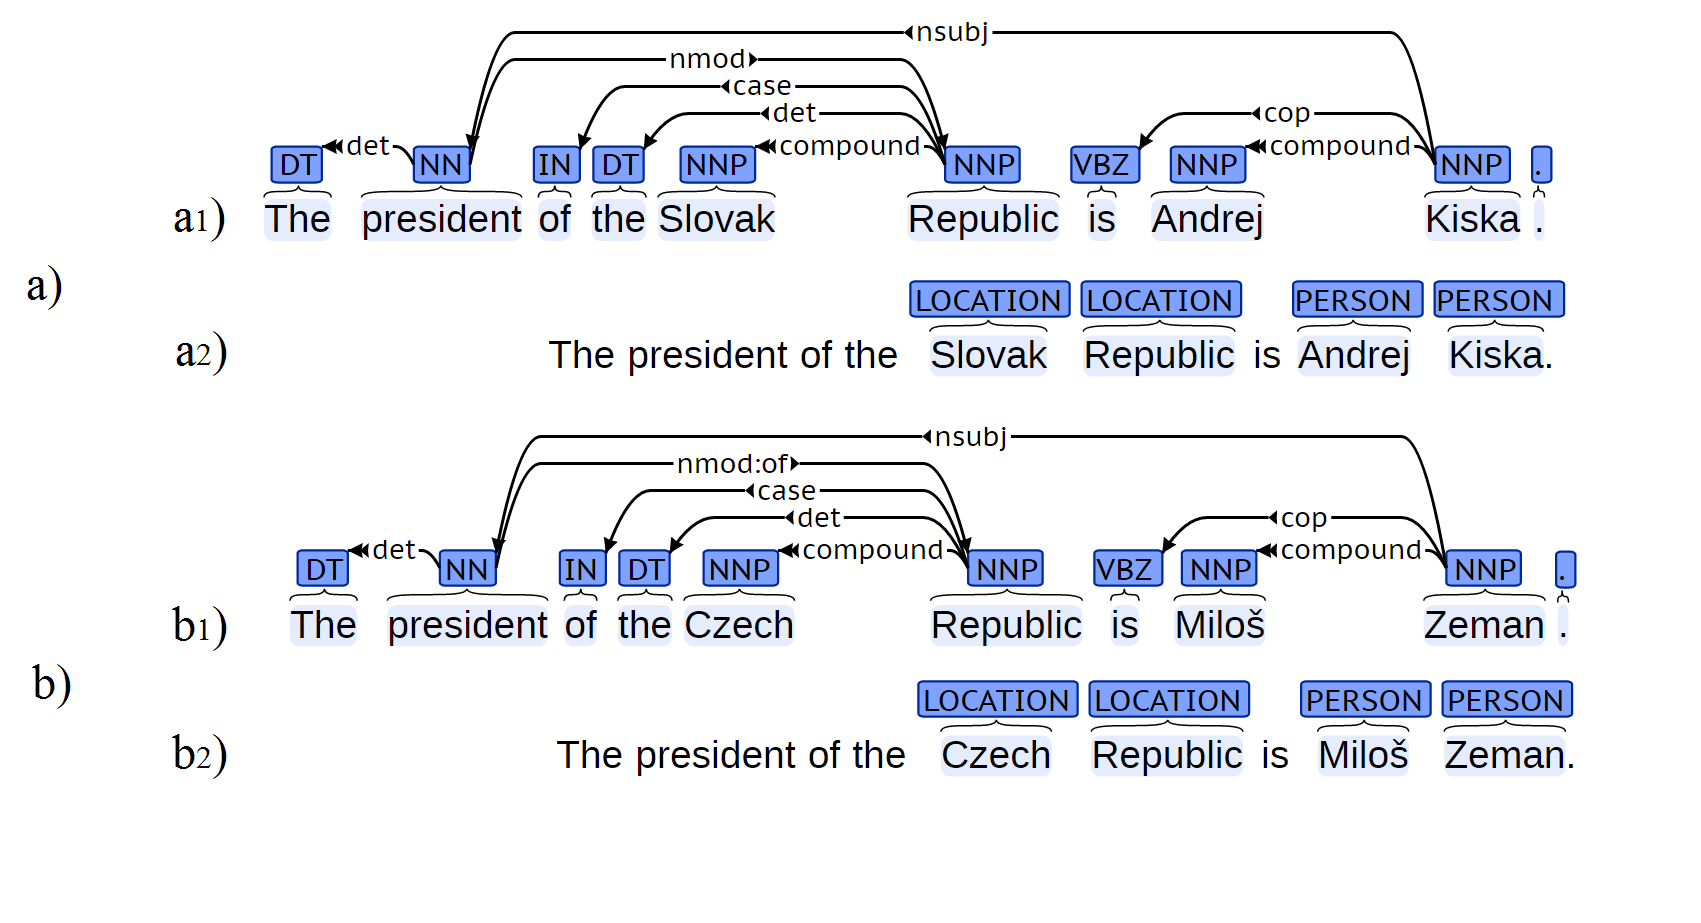
\includegraphics[scale=0.33]{calculate_sentences_match_example}\end{center}
	\caption[Príklad určenia zhody viet]{Príklad určenia zhody viet}\label{fig:calculate_match_sentences_example}
\end{figure}

Predpokladajme situáciu z obrázka~\fullref{fig:calculate_match_sentences_example}. V databáze máme uloženú spracovanú vetu \textit{a} aj s pravidlom pre túto vetu. Spracovávame vetu \textit{b}. Na časti \textit{a1} obrázka~\fullref{fig:calculate_match_sentences_example} sú znázornené závislostí a na časti \textit{a2} názvoslovné entity vety \textit{a}. Na časti \textit{b1} sú znázornené závislostí a na časti \textit{b2} názvoslovné entity vety \textit{b}. V tejto situácií potrebujeme vypočítať zhodu medzi vetami \textit{a} a \textit{b}. 

Pri štrukturálnej časti zhody sa prechádza cez všetky závislosti vety \textit{a}. Prvá závislosť je závislosť so vzťahom \textit{DET} a nadradeným tokenom s nadradenou značkou slovného druhu \textit{NN} a podradeným tokenom s nadradenou značkou slovného druhu \textit{DT}. V prom kroku sa pozrie, či veta \textit{b} obsahuje ľubovoľnú závislosť s podradeným tokenom s nadradenou značkou slovného druhu \textit{DT}. V ďalšom kroku, sa zistí, či veta \textit{b} obsahuje ľubovoľnú závislosť s nadradeným tokenom s nadradenou značkou sloveného druhu \textit{NN}. Môže to byť aj iná závislosť, ako tá z prvého kroku. Pokračuje sa zistením úplnej zhody závislosti. Určí sa , či veta \textbf{b} obsahuje ľubovoľnú závislosť s podradeným tokenom s nadradenou značkou slovného druhu práve \textit{DT} a zároveň s nadradeným tokenom s nadradenou značkou slovného druhu \textit{NN}. Takto sa iteruje cez všetky závislosti vety \textit{a}. Na záver sa určí zhoda počtu závislostí s rovnakou štruktúrou. Napríklad veta \textit{a} obsahuje práve dve závislosti, ktoré majú na podradenom tokene nadradenú značku slového druhu \textit{DT} a na nadradenom tokene nadradenú značku slovného druhu \textit{NN}. Zistí sa, či aj veta \textit{b} obsahuje práve dve takéto závislosti. \\

Prvá závislosť vo vete \textit{b} je so vzťahom \textit{det}, nadradeným tokenom so značkou slovného druhu \textit{NN} a indexom 1 a podradeným tokenom so značkou slovného druhu \textit{DT} a indexom 0. Token slova \textit{Slovak} má názvoslovnú entity typu \textit{LOCATION - lokácia}. Ak slovo nemá vyobrazený typ názvoslovnej entity, znamená to, že má názvoslovnú entity typu \textit{OTHER - ostatné}. V prvok kroku pri určovaní obsahovej časti zhody zisťujeme, či veta \textit{b} obsahuje závislosť so vzťahom \textit{det} a tokenmi so značkou slovného druhu \textit{NN} alebo \textit{DT} a indexmi rovnými 0 alebo 1. Toto je separátny výpočet značiek slovných druhov a indexov. V tomto isto kroku sa tiež pozrie, či veta \textit{b} obsahuje ľubovoľnú závislosť s podradeným tokenon s názvoslovnou entitou typu \textit{ostatné} (názvoslovná entita tokenu \textit{THE} vo vete \textit{a}) a ľubovoľnú závislosť s nadradeným tokenom s názvoslovnou entitou typu \textit{ostatné} (názvoslovná entita tokenu \textit{president} vo vete \textit{a}). V nasledujúcom kroku zisťujeme, či veta \textit{b} obsahuje závislosť so vzťahom \textit{det} a nadradeným alebo podradeným tokenom so značkou slovného druhu \textit{NN} a indexom 1 alebo značkou slovného druhu \textit{DT} a indexom 0. Toto je polovičná zhoda. V poslednom kroku hľadáme vo vete \textit{b} závislosť so vzťahom \textit{det} a nadradeným tokenom práve so značkou slovného druhu \textit{NN} a indexom 1 a zároveň podradeným tokenom práve so značkou slovného druhu \textit{DT} a indexom 0. Zároveň v tomto kroku sa zisťuje, či veta \textit{b} obsahuje závislosť s podradeným tokenom s názvoslovnou entitou typu \textit{ostatné} a zároveň s nadradeným tokenom s názvoslovnou entitou typy \textit{ostatné}. Iterácia pokračuje s nasledujúcou závislosťou, pokým sa nevyhodnotia všetky. \\

Pri určení hodnotovej časti zhody sa porovnajú texty \textit{,,The president of the Slovak Republic is Andrej Kiska.''} a \textit{,,The president of the Czech Republic is Miloš Zeman.''} a určí sa, či su zhodné. \\

Aplikovaním určenia zhody viet medzi vetami \textit{a} a \textit{b} zistíme, že veta \textit{b} má štrukturálnu časť zhody s vetou \textit{a} $100\%$. Tak isto má obsahovú časť zhody rovnú $100\%$. Hodnotová časť zhody je $0\%$.

%
% Nadradená značka slovného druhu
%
\ifthenelse {\boolean{bachelor}}
{
	%\subsection{Subsection}
	\paragraph{Nadradená značka slovného druhu}
}
{
	%\section{Subsection}
	\subsubsection{Nadradená značka slovného druhu}
}
\label{paragraph:superior_pos_tag}

Pod nadradenou značkou slovného druhu sa chápe značka slovného druhu zoskupujúca množinu značiek slovných druhov, do ktorej značka slovného druhu patrí. 

Napríklad značka slovného druhu VBD (Verb, past tense - sloveso v minulom čase) patrí medzi skupinu značiek slovných druhov slovies \textit{\{VB, VBD, VBG, VBN, VBP, VBZ\}}. Z toho vyplýva, že nadradená značka slovného druhu \textit{VBD} je VB (Verb - sloveso).

%
% Aplikovanie pravidla
%
\ifthenelse {\boolean{bachelor}}
{
	%\subsection{Subsection}
	\subsubsection{Aplikovanie pravidla}
}
{
	%\section{Subsection}
	\subsection{Aplikovanie pravidla}
}
\label{subsubsection:rule_application}

Procesom vyhľadania pravidla (viď.~\fullref{subsubsection:rule_lookup}) sme získali pravidlo na spracovanie vety. Aplikáciou pravidla na vetu vytvoríme poznámku.

Proces aplikovania pravidla na vetu s cieľom vytvorenia poznámky má viacero krokov. Pre všetky závislosti zo \textit{zoznamu dát štruktúry} pravidla, príslušná závislosť je vyhľadaná v spracovávanej vete. Pri vyhľadávaní príslušnej závislosti sa závislosti neporovnávajú, okrem iného, na základe značiek slovných druhov svojich tokenov, ale podľa nadradených značiek slovných druhov (viď.~\nameref{paragraph:superior_pos_tag} na strane~\pageref{paragraph:superior_pos_tag}) svojich tokenov. Tento spôsob vyhľadávania nám umožňuje [BLA BLA, blizie opisane v BLA BLA]. Avšak, môže to spôsobiť vyhľadanie viac ako jednej príslušnej závislosti. Preto musí byť vypočítaná zhoda závislostí (viď.~\nameref{paragraph:dependency_match} na strane \pageref{paragraph:dependency_match}). Po vypočítaní zhody závislostí a získanie závislosti s najväčšou zhodou, slovo korešpondujúce s tokenom, ktorý sa ma z danej závislosti vybrať, sa pridá do poznámky na pozíciu pozície závislosti. Po spracovaní všetkých závislostí, posledné minoritné úpravy sú vykonané nad poznámkou, ako rozdelenie na viacero viet, ak tak určovalo pravidlo, kapitalizácia prvých písmen viet poznámky a iné. Pseudokód aplikovania pravidla na vetu s cieľom vytvoriť poznámku je zobrazený na algoritme~\ref{alg:applying_rule}.

\begin{algorithm}
	\floatname{algorithm}{Algoritmus}
	\caption[Aplikovanie pravidla]{Aplikovanie pravidla}\label{alg:applying_rule}
	\begin{algorithmic}[1]
		\Procedure{ApplyRule}{$sentence, rule$}
		\State $note \gets \text{new Note}$
		\ForAll {$ruleDependencies$}
		\State $dependency \gets \text{findDependency(} sentence \text{, } ruleDependency \text{)}$
		\If {$\text{isFound(}dependency\text{)}$}
		\State $\text{add(} note \text{, getDependent(} dependency \text{))}$
		\If {$\text{isNominalSubject(relation(}dependency \text{))}$}
		\State $\text{add(} note \text{, getGovernor(} dependency \text{))}$
		\EndIf
		\EndIf
		\EndFor
		
		\State $\text{splitToSentences(} note \text{, sentencesEnds(} rule \text{))}$	
		
		\Return $note$
		\EndProcedure
	\end{algorithmic}
\end{algorithm}

Pre vetu \textit{,,The president of the Slovak republic is Andrej Kiska.''} nám nástroj Stanford CoreNLP poskytne závislostí vyobrazené na obrázku~\fullref{fig:example_sentence_andrej_kiska}. Ak na túto vetu aplikujeme pravidlo so štruktúrou v tvare zobrazenej na obrázku~\fullref{fig:apply_rule_example_rule}, výsledná poznámka bude \textit{,,President is Kiska.''}. 

Aplikovanie pravidla prebieha nasledovným spôsobom. Prechádzajú sa všetky závislosti v štruktúre pravidla. Prvá závislosť v štruktúre pravidla je závislosť so vzťahom \textit{nsubj} na pozícií jedna a podradeným korešpondujúcim tokenom. Má podradený token so značkou slovného druhu \textit{NN}, typom názvoslovnej entity \textit{OTHER - ostatné}, lemou \textit{President} a indexom dva. Nadradený token má značku slovného druhu \textit{NNP}, názvoslovnú entitu \textit{PERSON - osoba}, lemu \textit{Kiska} a index deväť. Takáto závislosť sa vyhľadá v štruktúre vety medzi závislosťami na obrázku~\fullref{fig:example_sentence_andrej_kiska}. Ak pre danú závislosť vyhovuje viacero závislostí, pomocou výpočtu zhody závislostí vyberieme tú s najväčšou zhodou. V tomto prípade vidíme, že vyhovujúca závislosť je len jedna a to prvá závislosť \textit{nsubj} medzi slovom na druhej pozícií \textit{president} a posledným slovom, na deviatej pozícií \textit{Kiska}. Z tejto závislosti sa zoberie podradený token, keďže tak určuje pravidlo v stĺpci \textit{typ tokenu}. Slovo \textit{president} sa pridá do poznámky na pozíciu jedna. Rovnakým spôsobom sa prechádzajú a spracujú všetky závislosti v štruktúre pravidla a podľa nich sa extrahuje slovo z vety a pridá do poznámky.

\begin{figure}[H]
	\begin{center}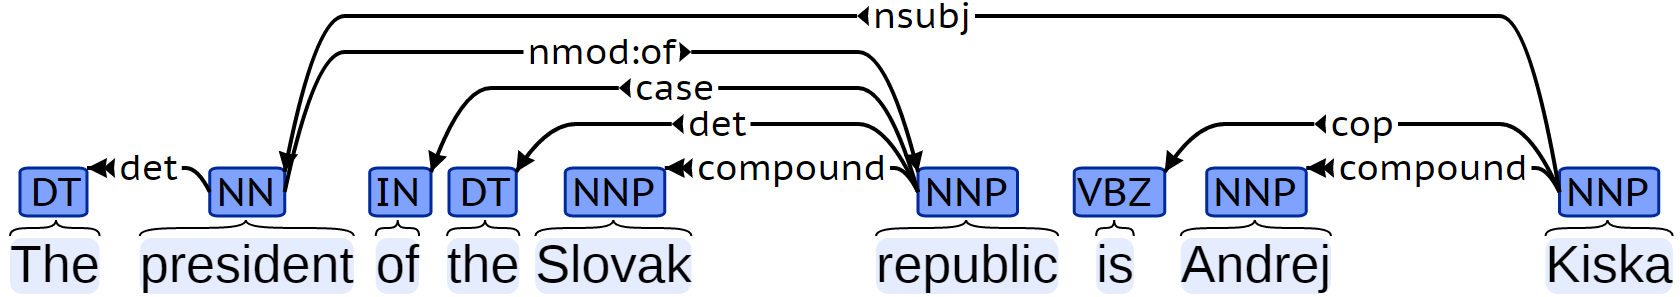
\includegraphics[scale=0.32]{example_sentence_andrej_kiska}\end{center}
	\caption[Zásivlostí jednoduchej vety]{Zásivlostí jednoduchej vety}\label{fig:example_sentence_andrej_kiska}
\end{figure}

\begin{figure}[H]
	\begin{center}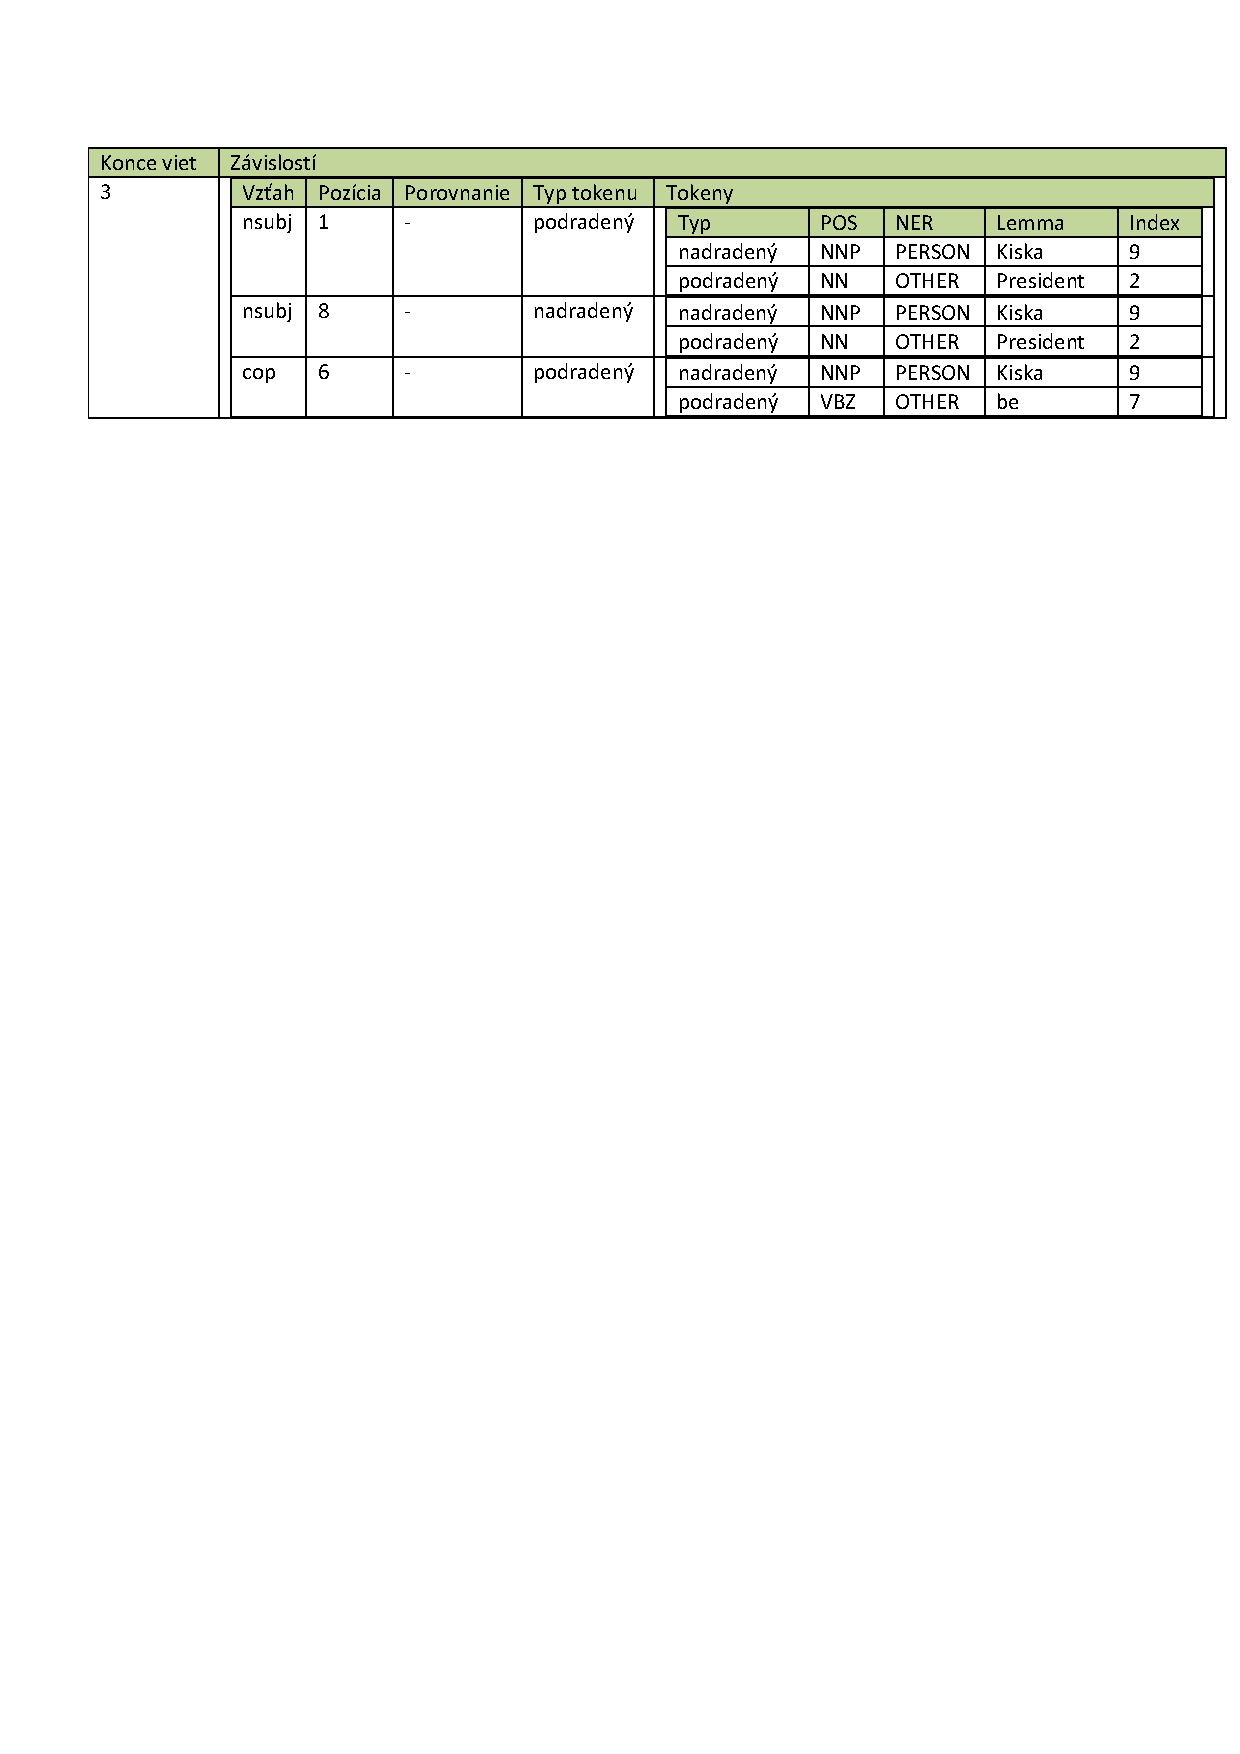
\includegraphics[scale=0.32]{apply_rule_example_rule}\end{center}
	\caption[Príklad štruktúry pravidla]{Príklad štruktúry pravidla}\label{fig:apply_rule_example_rule}
\end{figure}

%
% Výpočet zhody závislostí
%
\ifthenelse {\boolean{bachelor}}
{
	%\subsection{Subsection}
	\paragraph{Výpočet zhody závislostí}
}
{
	%\section{Subsection}
	\subsubsection{Výpočet zhody závislostí}
}
\label{paragraph:dependency_match}

Princíp výpočtu zhody závislostí je veľmi podobný s výpočtom zhody viet zo sekcie~\fullref{subsubsection:rule_lookup}. Porovnávajú sa vždy nadradené aj podradené tokeny. Porovnanie má niekoľko krokov. Začína sa s porovnaním značiek slovných druhov. Pokračuje sa názvoslovnou entitou, indexom, lemou a nakoniec sa porovnáva vzdialenosť pozícií tokenov vo vetách. Každý krok je príslušne ohodnotený a ak porovnanie bolo úspešné, ohodnotenie sa pripočíta k finálnej hodnote reprezentujúcej percentuálnej zhody závislostí.

%
% Vytváranie pravidla
%
\ifthenelse {\boolean{bachelor}}
{
	%\subsection{Subsection}
	\subsubsection{Vytvorenie pravidla}
}
{
	%\section{Subsection}
	\subsection{Vytvorenie pravidla}
}
\label{subsubsection:rule_creation}
Ak nám proces vyhľadania pravidla nevyhľadal žiadne pravidlo, znamená to, že sme doposiaľ nespracovávali takú istú alebo podobnú vetu. V tomto prípade sú použité statické pravidlá na spracovanie vety. Výstupom bude zjednodušená veta - poznámka.

Vytvorí sa záznam o pôvodnej vete, ktorý okrem iného obsahuje \textit{zoznam dát o pôvodnej vete}, ktorý sa vyskladá zo závislostí vety. Následne sa vytvorí záznam o pravidle, ktorý okrem iného obsahuje \textit{zoznam dát o poznámke}, vyskladaný zo závislosti poznámky. Nakoniec sa tieto dva záznamy prepoja a tým sa vytvorí nové pravidlo na spracovanie takej istej alebo podobnej vety, akú sme práve spracovali.

%Na obrázku~\fullref{fig:rule_creation} je znázornený proces nevyhľadania pravidla, použitia parsera s následným uložením nového pravidla.

%\begin{figure}[H]
%	\begin{center}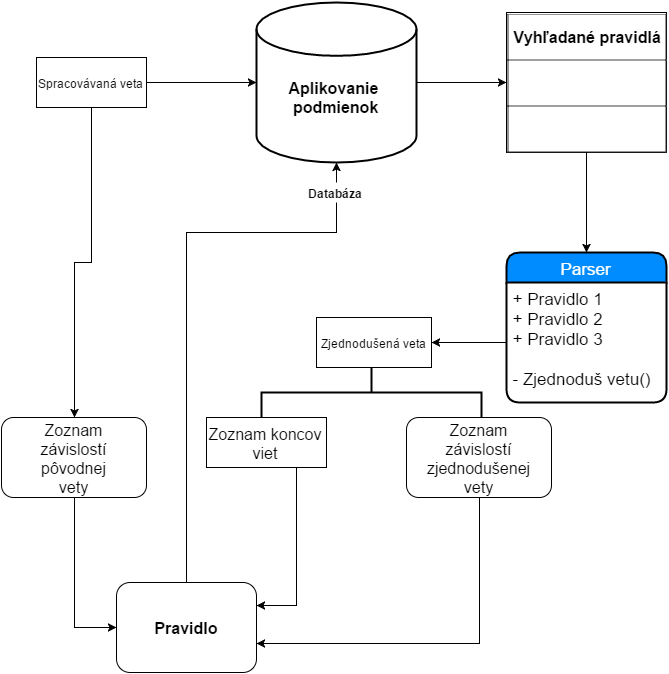
\includegraphics[scale=0.5]{rule_creation}\end{center}
%	\caption[Vytvorenie pravidla]{Vytvorenie pravidla}\label{fig:rule_creation}
%\end{figure}